\documentclass[12pt]{article}
\usepackage{sbc-template}
\usepackage[alf]{abntex2cite} 
\usepackage{graphicx,url}
\usepackage[utf8]{inputenc}
\usepackage[brazil]{babel}
%\usepackage[latin1]{inputenc}      %Erro no inputenc.

\sloppy

\title{O Professor como Coordenador em um Jogo para Prevenção da Violência Sexual Infantil}

\author{Alexandre Mendonça Fava\inst{1}, Carla Diacui Medeiros Berkenbrock\inst{1}}
%\author{Avaliação Cega\inst{1}, Avaliação Cega\inst{2}}


\address{\inst{}Universidade do Estado de Santa Catarina - UDESC\\Programa de Pós-graduação em Computação Aplicada - PPGCA\\Joinville - SC - Brasil CEP: 89.219-710
    \email{\{alexandre.fava@hotmail.com, carla.berkenbrock@udesc.br\}}
}

%\address{\inst{,2}Avaliação Cega
%    \email{\{Avaliação Cega\inst{1}, Avaliação Cega\inst{2}\}}
%}

\begin{document} 

\maketitle

\vspace{-0.2cm}

\begin{abstract}
Child Sexual Abuse is a worldwide issue which injures the victims and the society. This fact is responsible for the development of some methods of prevention of sexual abuse of children. In this sense, the current research presents a serious game aimed at instructing children against sexual violence. A game-based approach is a powerful learning tool as it promotes a fun and engaging educational environment. In addition to child learning, the game developed also provides a supporting platform for teachers, making them the game coordinator.
\end{abstract}

\vspace{-0.5cm}

\begin{resumo} 
O abuso sexual infantil é um problema de saúde pública mundial que prejudica suas vítimas e a sociedade. Em resposta a esse problema, programas de prevenção da violência sexual infantil têm sido desenvolvidos. Nesse sentido, a atual pesquisa apresenta um jogo sério com o intuito de instruir as crianças contra a violência sexual. Uma abordagem baseada em jogos é uma poderosa ferramenta de ensino na medida em que promove um ambiente educacional envolvente. Além da aprendizagem infantil, o jogo desenvolvido também fornece uma plataforma de apoio ao professor, tornando-o coordenador do jogo.
\end{resumo}

\vspace{-0.2cm}

\section{Introdução}\label{secao:introducao}

A violência infantil é um problema de saúde pública que resulta em inúmeras sequelas, prejudicando além das vítimas da violência, a sociedade como um todo. A criança violentada chega em sua fase adulta, apresentando os mais variados transtornos e distúrbios \cite{lima2018violencia}. A alta maleabilidade do encéfalo infantil permite que experiências negativas tenham maior probabilidade de causar efeitos graves e permanentes ao indivíduo \cite{pereira2011crescimento}. Um indivíduo sequelado em sua infância dificilmente alcançará seu verdadeiro potencial em sua fase adulta, deixando de colaborar de maneira significativa na sociedade, uma vez que tais indivíduos apresentam maior predisposição para alcoolismo, abuso de drogas, depressão e ideação suicida \cite{da2019violencia}.

Os maus-tratos contra as crianças são uma triste realidade em milhares de lares brasileiros. Em 2011 foram registradas 82.139 denúncias no Disque-100\footnote{O Disque 100 funciona diariamente, 24 horas por dia, incluindo sábados, domingos e feriados. Existem três opções para registrar sua denúncia: Disque 100, aplicativo Proteja Brasil e Ouvidoria Online (Disponível em: \url{https://www.humanizaredes.gov.br/ouvidoria-online/})}, já para o ano de 2017 a violência infantil totalizou 84.049 denúncias \cite{DireitosHumanos2018}. Os índices de violência infantil não demonstram  tendência de queda entre os anos de 2011 e 2017, o que aponta uma projeção alarmante para os próximos anos caso nenhuma medida seja tomada \cite{Boletim2018}.

Os casos de maus-tratos mais frequentemente denunciados são: Negligência, Violência Psicológica, Violência Física e Violência Sexual. O abuso sexual corresponde cerca de 20\% das violências registradas contra os menores, contudo tal abuso se classifica como uma das violações mais devastadoras \cite{hockenberry2011wong}. A violência sexual infantil assume uma condição única, apresentando quantitativamente números baixos (em relação as demais violações), entretanto qualitativamente um devastador impacto.


\section{Trabalhos Relacionados}\label{secao:trabalhos}

Diante do problema da violência sexual, estratégias nacionais como a Operação \textit{Darknet} da Polícia Federal surgiram, visando o fortalecimento das buscas e o encarceramento de criminosos \cite{Darknet2017}. Nacionalmente, surgiu também o jogo \textbf{Criança Protegida} que objetiva-se em instruir as crianças de modo que elas aprendam a se proteger de situações de violência \cite{carrara2018criancca}. 

A atual pesquisa introduz uma abordagem baseada em jogos para a prevenção do abuso sexual infantil. O jogo desenvolvido intitula-se \textbf{Infância Segura}, e visa seguir as orientações sobre sexualidade infantil definidas pela UNESCO \cite{women2018international}. O jogo \textbf{Infância Segura} precede o jogo \textbf{Criança Protegida} em termos cronológicos. Além disso, a revisão bibliográfica realizada anteriormente ao desenvolvimento do jogo não apresentou registros de estratégias similares no âmbito nacional, apenas em caráter internacional, como os jogos: \textit{Orbit}\footnote{\url{http://orbit.org.au/}}, 
\textit{Being Safety Smart}\footnote{\url{http://www.beingsafetysmart.com.au/}}, 
\textit{Child Abuse Prevention}\footnote{\url{https://androidappsapk.co/detail-child-abuse-prevention/}}.

As estratégias baseadas em jogos didáticos vêm a agregar e facilitar o aprendizado infantil, principalmente em temas difíceis de abordar, devido aos tabus e aos preconceitos  que os permeiam \cite{miranda2018abordagem}. O jogo \textbf{Infância Segura} apresenta-se como uma estratégia para reduzir a violência sexual infantil, uma vez que atua de maneira preventiva, diferentemente das estratégias corretivas da polícia. 


\section{Infância Segura}\label{secao:infancia}

O jogo Infância Segura foi idealizado e desenvolvido inicialmente por \citeonline{Tiago2018}. Contudo, o jogo em questão passou por uma série de modificações e melhorias que culminaram em duas aplicações distintas, uma voltada somente para os alunos (crianças) e a outra voltada somente para os professores (coordenadores). A versão voltada aos menores é tratada na subseção \ref{secao:jogo}, enquanto a versão voltada aos professores e pedagogos é tratada na subseção \ref{secao:coordenacao}.


\subsection{Jogo}\label{secao:jogo}

O jogo Infância Segura se aproxima de um Ambiente Virtual de Aprendizagem (AVA), o qual ministra conteúdos relacionados com a educação sexual infantil \cite{tarouco2009gestao}. O jogo foi desenvolvido considerando um público alvo de crianças a partir dos cinco anos de idade. Desta forma, o sistema de cadastro no jogo é simplificado em relação aos demais AVAs (como o \textit{Moodle}). Nesse sentido, os cadastros realizados pelas crianças assumem desde o início características de um jogo, com a criança tendo que preencher seu nome no sistema e selecionar um animal em uma lista de animais (animal esse que será o \textit{token} de identificação da criança). Uma vez cadastrada, para adentrar no jogo, a criança apenas precisa informar seu nome e seu \textit{token} para uma instrutora virtual.

A criança tem acesso ao jogo após informar seu gênero, entrar em uma turma, selecionar um personagem e escolher um amigo virtual. O personagem controlado pela criança obedece a dinâmica do herói mudo. Tal dinâmica é usada visando construir uma conexão mais forte entre personagem e jogador, descartando assim qualquer risco do personagem se utilizar de palavras ou de elementos contextuais que a criança desconheça \cite{domsch2017dialogue}. Nesse sentido, os elementos de narrativa são transferidos para um personagem que o jogador não possui controle (o amigo virtual), com o intuito de evitar assim, uma disrupção da interligação entre personagem e jogador. O amigo virtual é um personagem não jogável (NPC, \textit{Non-Player Character}) que acompanha o personagem escolhido pela criança no ambiente virtual. É o amigo virtual que apresenta todo o mundo virtual para o jogador, como ilustrado na Figura \ref{fig:ambientes}.

\vspace{-0.2cm}
\begin{figure}[ht]
\centering
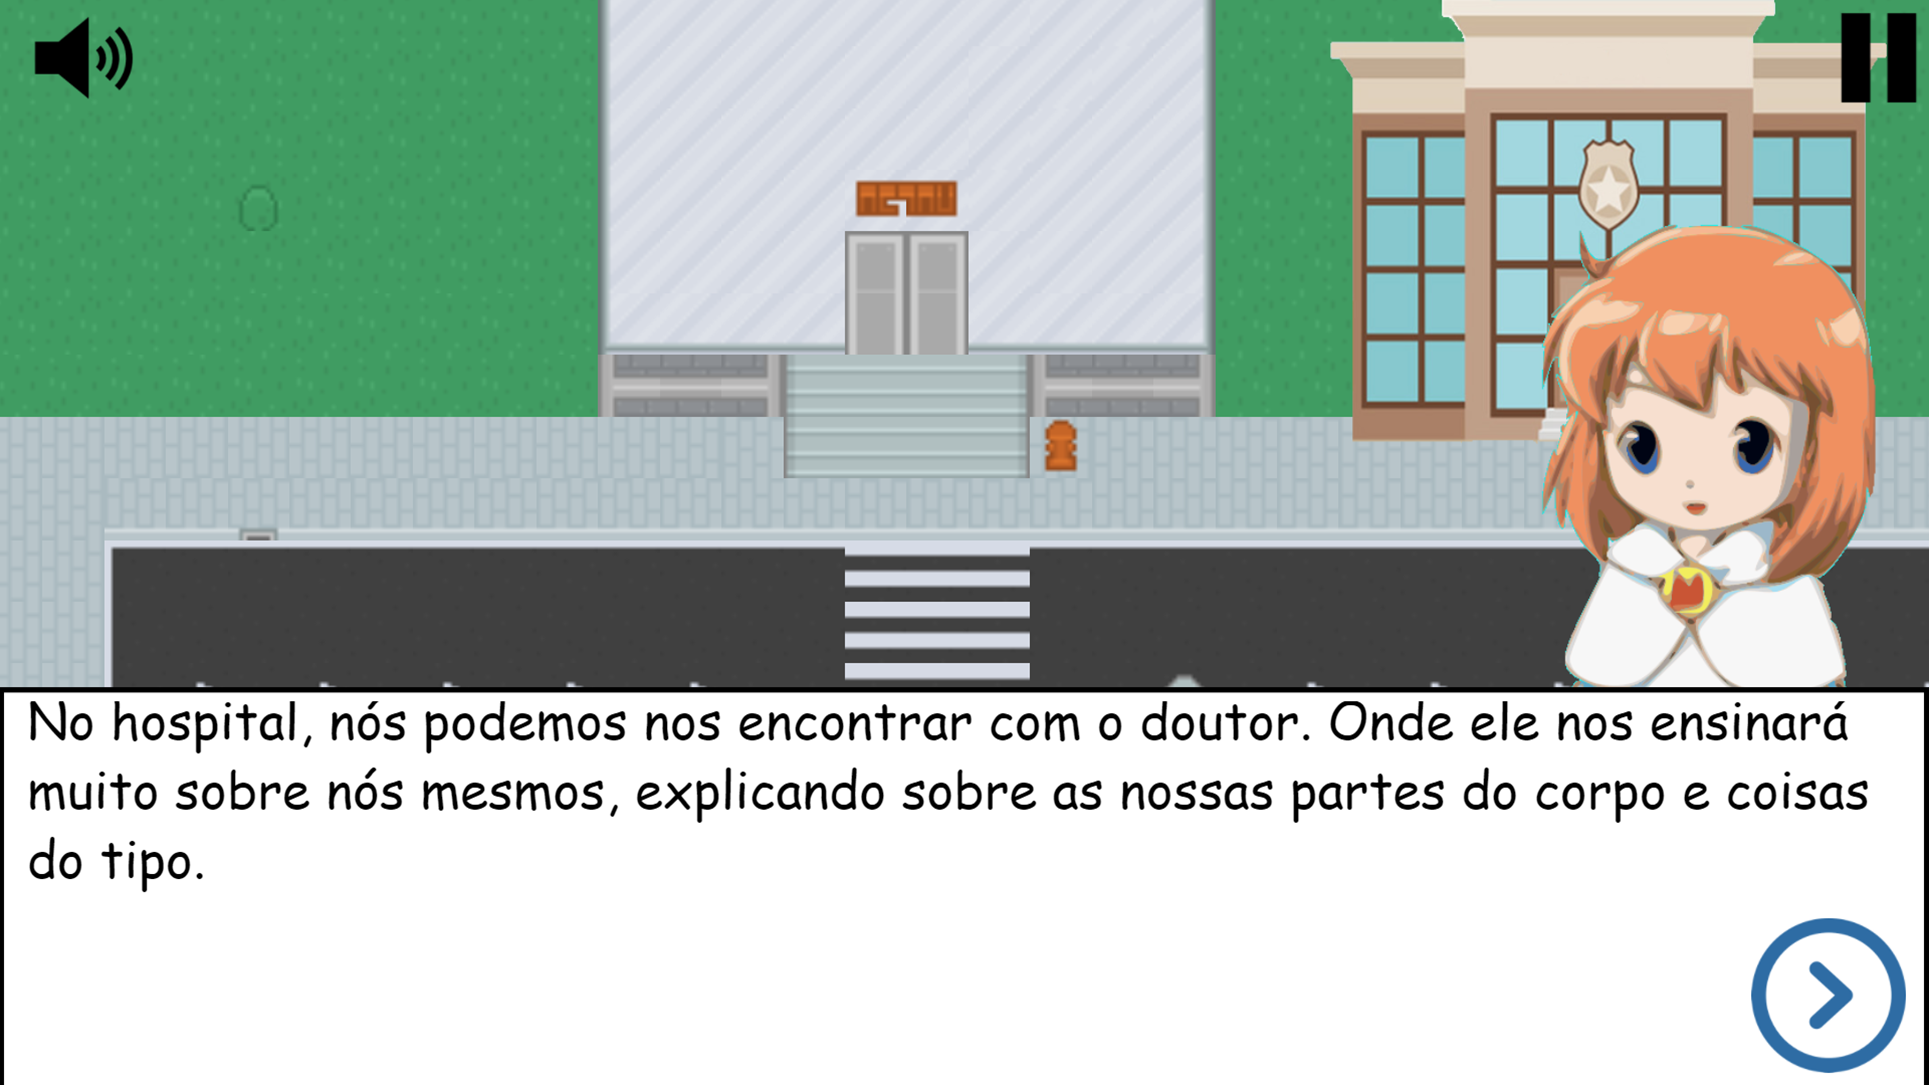
\includegraphics[width=.485\textwidth]{Figuras/Jogo/Hospital.png}
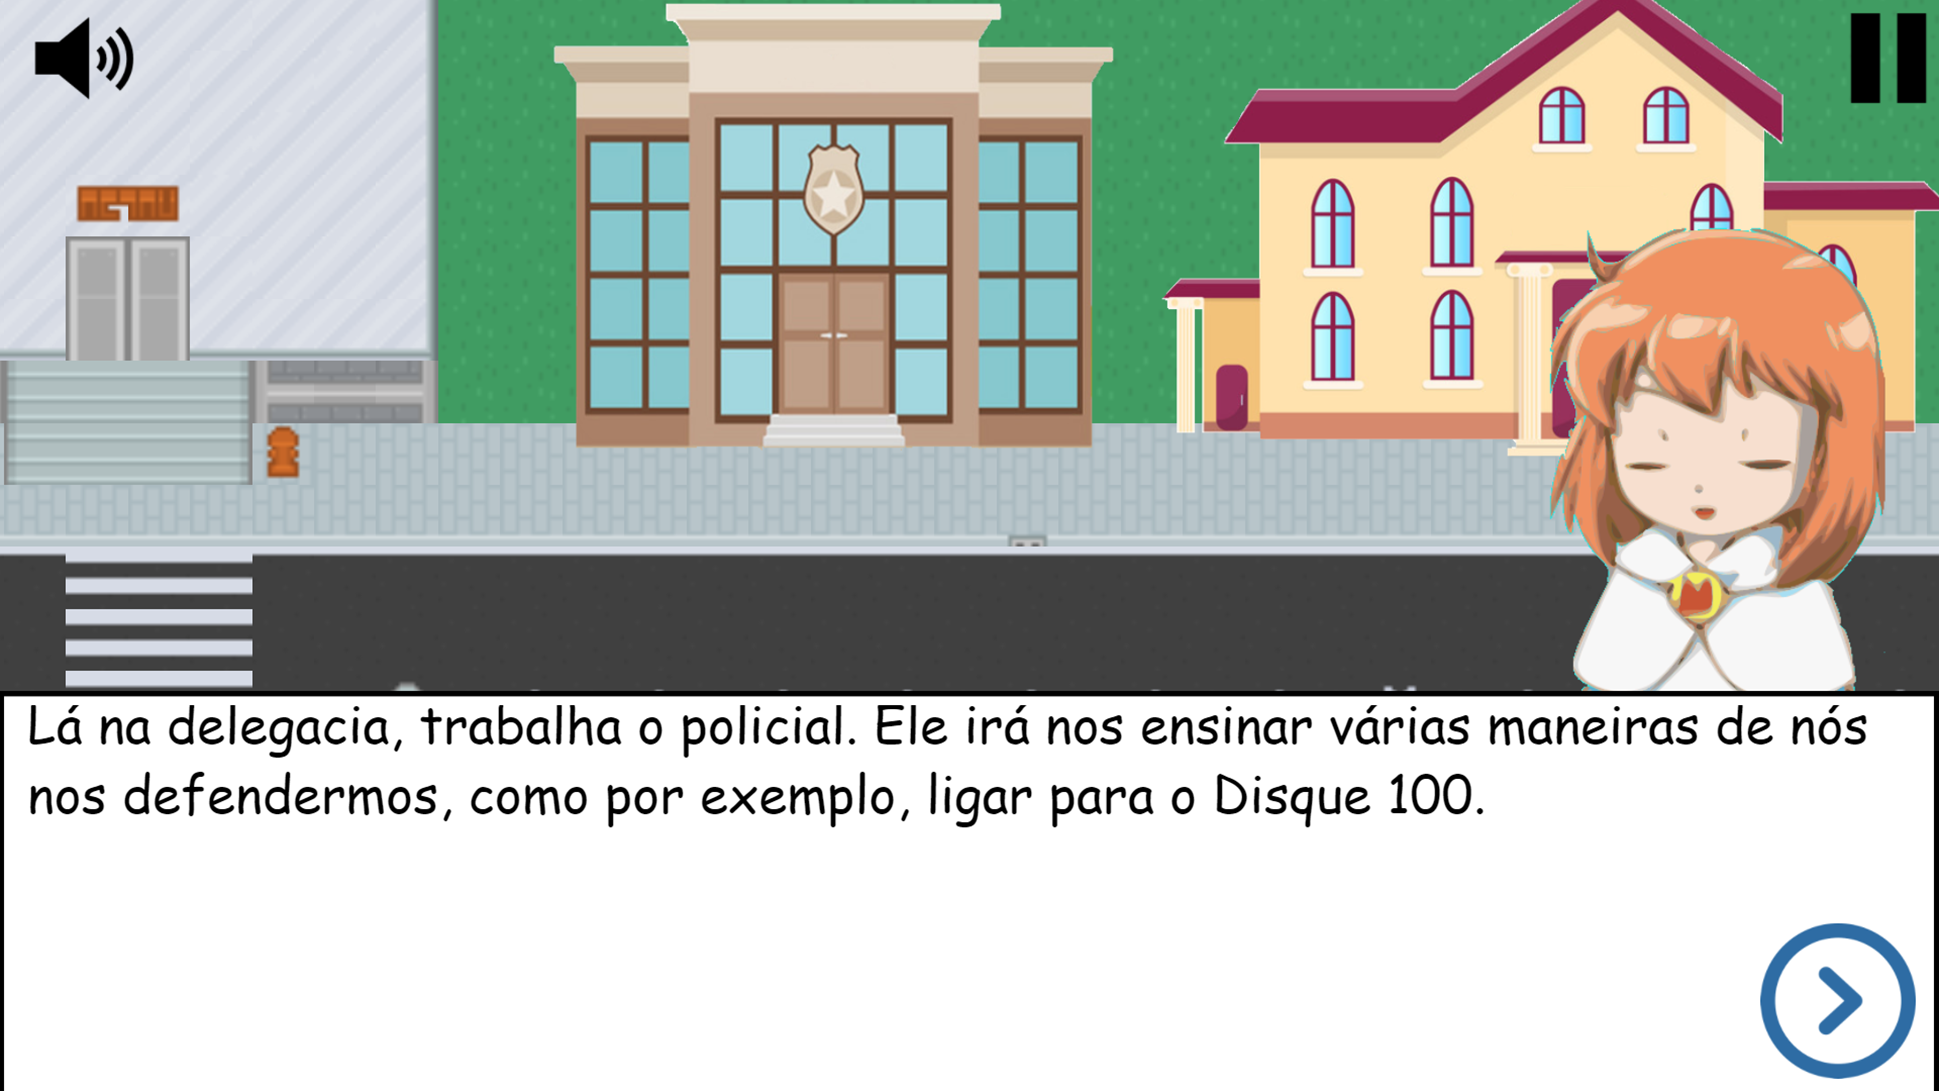
\includegraphics[width=.485\textwidth]{Figuras/Jogo/Delegacia.png}
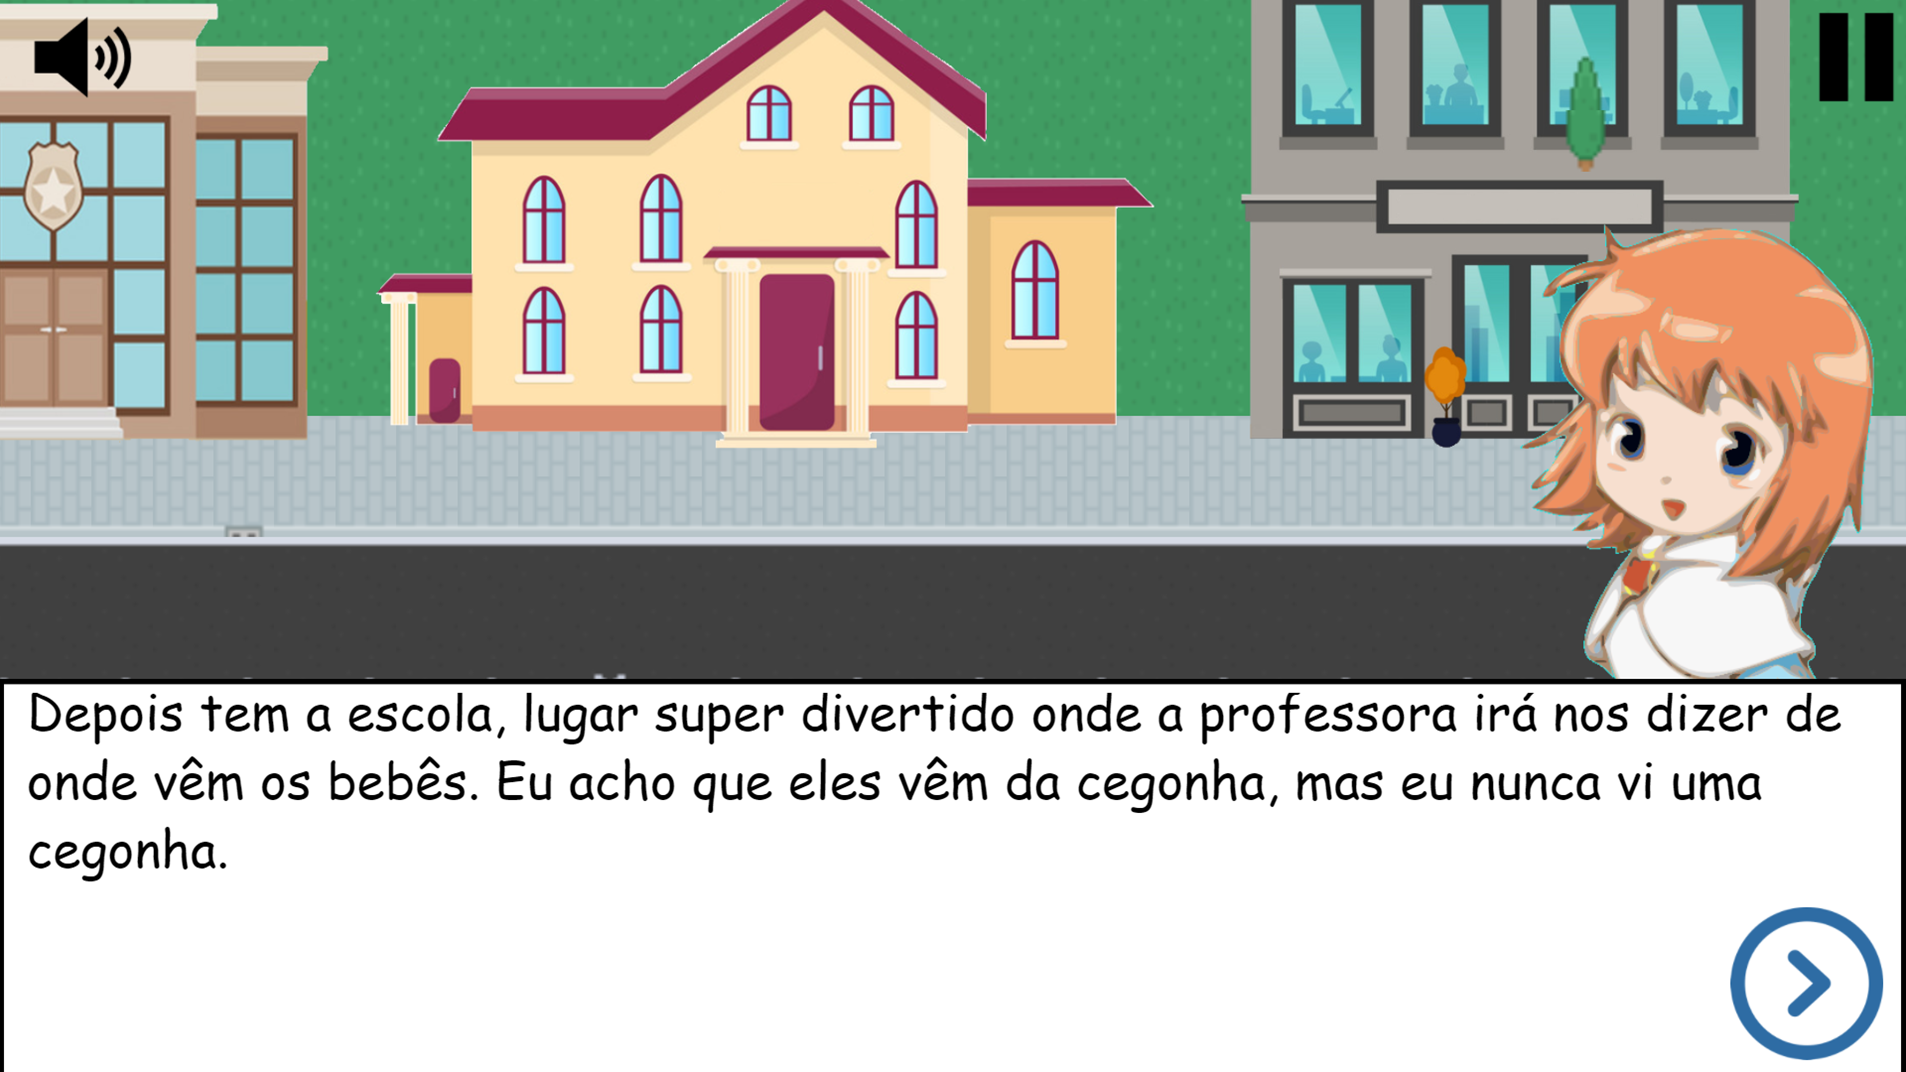
\includegraphics[width=.485\textwidth]{Figuras/Jogo/Escola.png}
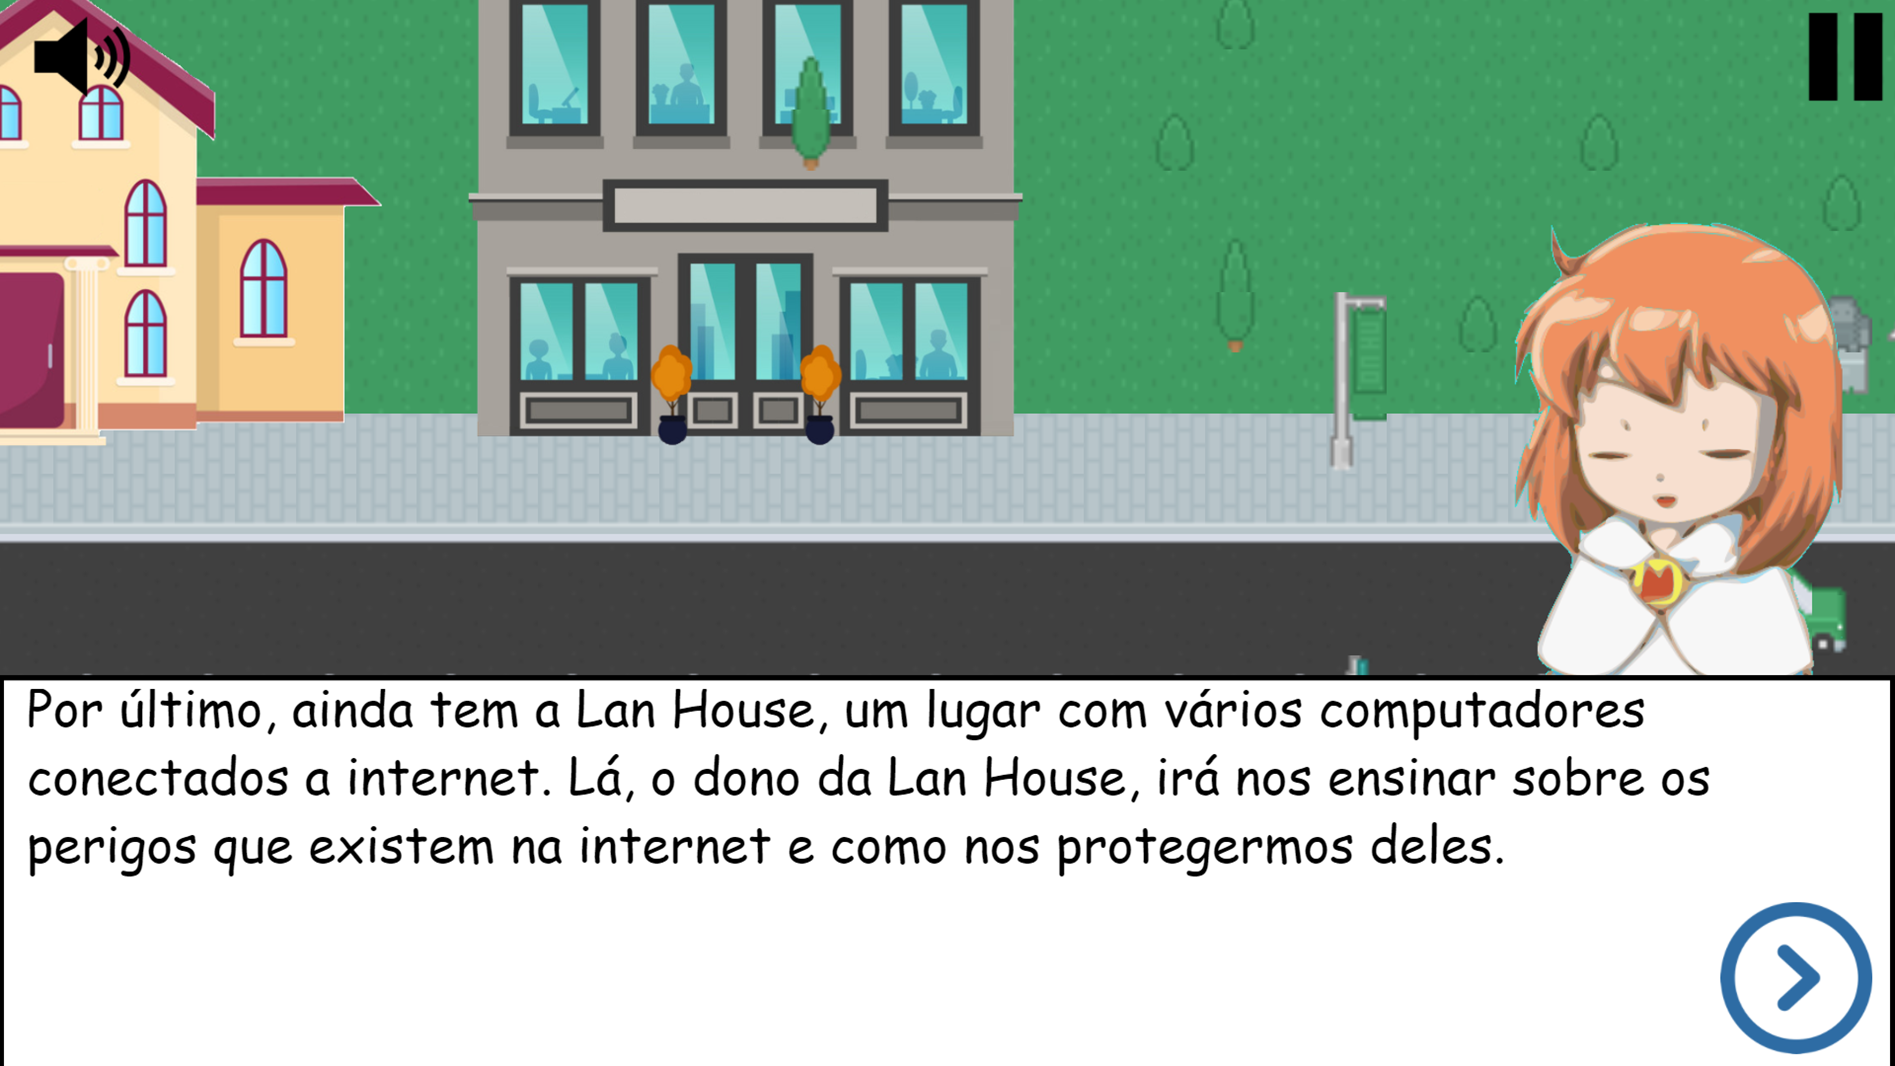
\includegraphics[width=.485\textwidth]{Figuras/Jogo/Lan-House.png}
\vspace{-0.2cm}
\caption{Telas dos Ambientes do jogo Infância Segura}
\label{fig:ambientes}
\end{figure}
\vspace{-0.2cm}

Nas quatro ilustrações da Figura \ref{fig:ambientes} a amiga virtual selecionada pelo jogador apresenta os ambientes do jogo. Na primeira tela da Figura \ref{fig:ambientes} é introduzido o Hospital, já na segunda tela é apresentada a Delegacia, na terceira tela a Escola e na quarta tela a Lan House. Cada local é apresentado brevemente, dando ao jogador uma vaga noção sobre as lições que são abordadas nos respectivos ambientes. O jogador é instruído tanto visualmente, quanto sonoramente, desta forma o jogo é capaz de abranger inclusive as crianças que não se encontram alfabetizadas. 

O jogador possui liberdade para vagar no mundo virtual com as setas direcionais apresentadas. Desta maneira a criança é capaz de adentrar nos ambientes e ter acesso aos seus conteúdos da forma que melhor lhe convir. Os materiais ministrados são independentes entre si, no entanto os conceitos a serem apresentados nos ambientes seguem uma hierarquia. No ambiente hospitalar, por exemplo, o jogador é primeiro ensinado sobre as partes do corpo, para em seguida aprender quais são suas partes íntimas, e posteriormente sobre os tipos de toques e quais atitudes tomar quando um toque ruim acontecer. 

Todas as ações realizadas pelas crianças durante as dinâmicas ministradas no jogo são enviadas para um banco de dados relacional. Dados sobre a quantidade de acertos, erros, e tempo preenchem os campos no banco de cada um dos jogadores. Os dados gerados pelo sistema não são apresentados ao jogador em nenhum momento. Tais informações são acessíveis apenas pelos professores na ferramenta destinada a coordenação.


\subsection{Coordenação}\label{secao:coordenacao}

O jogo Infância Segura permite o acesso ao banco de dados do sistema por meio de uma ferramenta de gestão colaborativa de conteúdo educacional. Nesse sentido a atual ferramenta se manifesta como um \textit{Learning Analytics} (LA) servindo como um instrumento auxiliador para a identificação e análise de dados \cite{prante2018professor}. Para acessar a plataforma o professor deve preencher um cadastro, onde são obrigatórios: nome, correio eletrônico, senha, escola, cidade e estado. Após estar cadastrado e devidamente autenticado, o professor tem acesso a plataforma apresentada na Figura \ref{fig:coordenador}.

\vspace{-0.2cm}
\begin{figure}[ht]
\centering
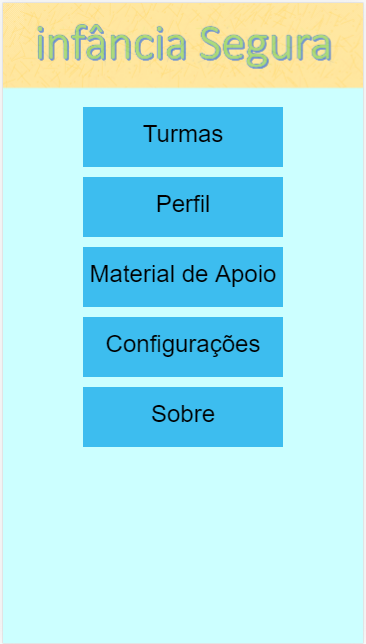
\includegraphics[width=.19\textwidth]{Figuras/Coordenacao/Prof-Menu.png}
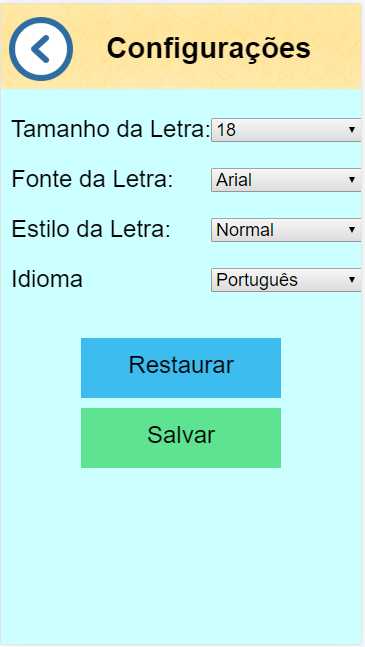
\includegraphics[width=.19\textwidth]{Figuras/Coordenacao/Prof-Configuracao.png}
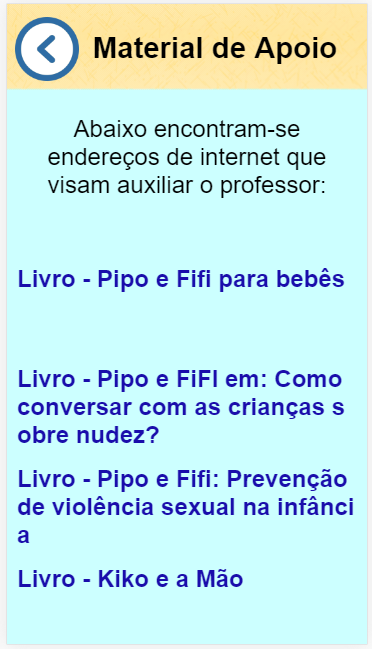
\includegraphics[width=.19\textwidth]{Figuras/Coordenacao/Prof-Material.png}
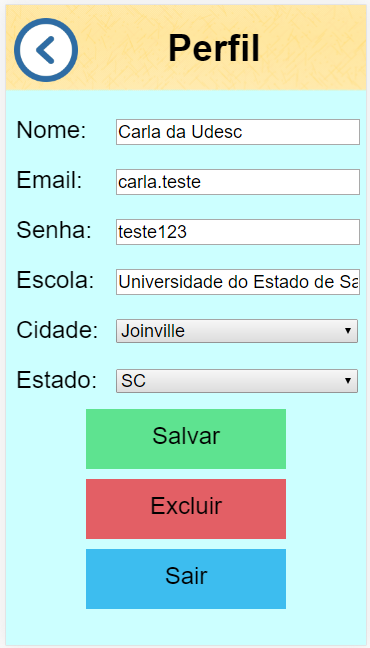
\includegraphics[width=.19\textwidth]{Figuras/Coordenacao/Prof-Perfil.png}\\
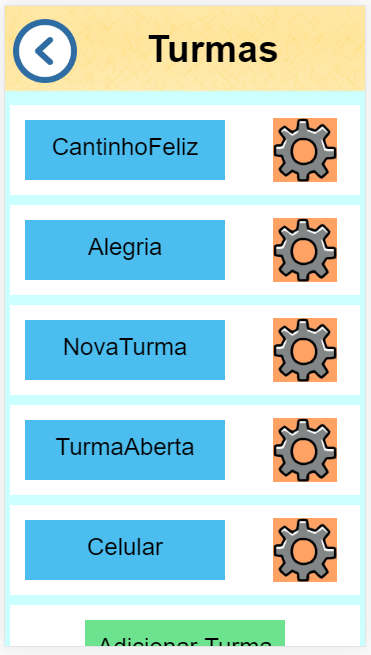
\includegraphics[width=.19\textwidth]{Figuras/Coordenacao/Prof-Turmas.png}
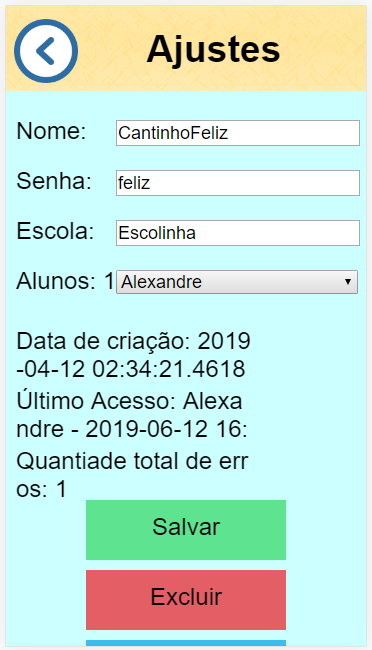
\includegraphics[width=.19\textwidth]{Figuras/Coordenacao/Prof-Ajustes.png}
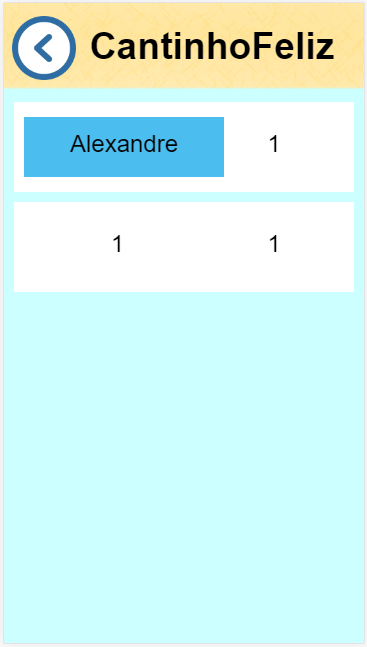
\includegraphics[width=.19\textwidth]{Figuras/Coordenacao/Prof-Alunos.png}
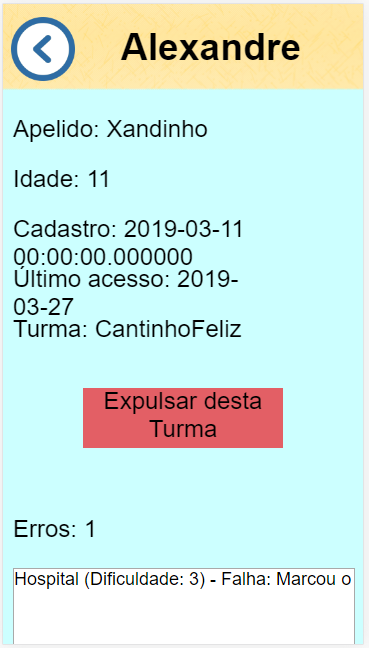
\includegraphics[width=.19\textwidth]{Figuras/Coordenacao/Prof-Aluno.png}
\vspace{-0.3cm}
\caption{Telas do Sistema do Coordenador}
\label{fig:coordenador}
\end{figure}
\vspace{-0.4cm}

Os \textit{layouts} da Figura \ref{fig:coordenador} são apresentados na versão \textit{mobile}, salienta-se no entanto que o sistema é responsivo, se adaptando as proporções do ecrã do coordenador. A primeira ilustração da Figura \ref{fig:coordenador} é apresentada ao usuário logo após ele se autenticar na plataforma. Nela o usuário é confrontado com as seguintes opções: Turmas, Perfil, Material de Apoio, Configurações e Sobre.

A opção \textbf{Turma} apresenta uma nova tela com todas as turmas que foram criadas para serem coordenadas. A seleção do \textbf{Perfil}, leva o usuário a uma nova tela, onde lhe é permitido a visualização e edição de suas informações. O botão \textbf{Material de Apoio} carrega uma lista de endereços em uma nova tela na aplicação. A opção \textbf{Configurações} redireciona o usuário a um \textit{layout} com capacidades de configuração e personalização. A opção \textbf{Sobre}, quando pressionada, carrega uma breve descrição sobre a aplicação.

No sistema em questão, o coordenador possui total liberdade para criar e gerenciar suas turmas. Uma vez que uma turma tenha sido cadastrada no sistema, as crianças podem se inscrever na turma. Ao selecionar uma turma, o professor tem acesso a lista dos alunos cadastrados naquela turma, e ao selecionar um aluno, o professor é confrontado com algumas informações geradas pelo aluno selecionado durante sua jogatina, como: data de cadastro, quantidade de erros, quantidade de acertos, descrição dos erros e acertos.


\subsection{Continuação da Pesquisa}\label{secao:continuacao}

O jogo Infância Segura desenvolvido apoia-se em um dos pilares fundamentais do Modelo 3C: a Coordenação. O Modelo 3C é frequentemente usado pela literatura para classificar os sistemas colaborativos, isso pois para existir a colaboração os indivíduos precisam trocar informações (Comunicação), organizar-se (Coordenação) e operar em conjunto num espaço compartilhado (Cooperação) \cite{pimentel2006modelo}.

A corrente versão do jogo foi ministrada a um grupo de crianças. Visando a análise do jogo, utilizou-se um questionário baseado no modelo teórico de \citeonline{savi2011avaliaccao}. A valoração dos itens do questionário foi medida na escala \textit{Likert} (valorada de -2 até 2), nesse sentido aponta-se que a média dos itens alcançou a marca de 1,6. Durante os testes os menores manifestaram grande entusiamos no jogo. Dentre as melhorias apontadas, destaca-se a necessidade de um botão para a releitura dos diálogos.

Em virtude da temática sensível do conteúdo abordado, questiona-se a inserção de um canal de interação entre os alunos, agregando assim a Comunicação ao sistema. Além da preocupação com o \textit{bullying} virtual, sabe-se que a interação e a colaboração entre os alunos em ambiente virtuais educativos é baixa \cite{aires2017estudo}. Nesse sentido busca-se o intercâmbio de ideias para uma eventual implementação da comunicação no jogo Infância Segura, pois questiona-se os reais benefícios na comunicação entre as crianças em um tema bastante íntimo. Salienta-se no entanto, que a implementação de um canal de comunicação entre os coordenadores e entre a criança e seu coordenador já está em curso. No âmbito do professor, destaca-se que a corrente versão da plataforma permite apenas a gestão dos alunos e não do conteúdo, contudo futuramente pretende-se implementar o gerenciamento de conteúdo para o coordenador (em nível limitado).

A atual pesquisa também encontra dificuldades na implementação de um jogo cooperativo na temática sobre a prevenção da violência sexual infantil. As estratégias conjecturadas se classificam mais como competitivas do que cooperativas, focando-se apenas em competições baseadas em tempo. Acredita-se que o intercurso de ideias ajudaria a encontrar soluções cooperativas viáveis de serem implementadas. 


\section{Conclusão}\label{secao:conclusao}

A violação sexual de direitos de crianças e adolescentes interfere diretamente no desenvolvimento da sexualidade saudável e nas dimensões psicossociais da criança e do adolescente, causando danos muitas vezes irreversíveis. Nesse sentido estratégias de prevenção e educação infantil se apresentam como uma forma de combater a violência sexual.

O jogo Infância Segura visa instruir as crianças contra a violência sexual. Atualmente o jogo encontra-se em fase de desenvolvimento, sendo este o momento ideal para sua apresentação a comunidade científica, visando assim o debate e o intercâmbios de ideias na área de sistemas colaborativos.

\section*{Agradecimentos}\label{secao:agradecimentos}

O presente trabalho foi realizado com apoio da Coordenação de Aperfeiçoamento de Pessoal de Nível Superior - Brasil (CAPES) - Código de Financiamento 001.

\vspace{-0.3cm}

%\bibliographystyle{sbc}
\bibliography{sbc-template}

\end{document}